\chapter{Implementation}

\section{Introduction}
This chapter presents the implementation details of the Echora system, describing how the
proposed design and requirements are realized in a practical, working prototype. It focuses
on the datasets, development environment, core algorithms, and system integration strategies
used to transform the conceptual architecture into an operational AI-powered sensory
substitution system.

The implementation emphasizes real-time performance, modularity, and on-device processing
to meet the strict latency, privacy, and reliability requirements defined in earlier chapters.
All computationally intensive tasks, including computer vision, depth processing, sensor
fusion, and machine learning inference, are executed locally on the mobile device, ensuring
independence from cloud connectivity and preserving user privacy.

This chapter begins by describing the datasets used to train and evaluate the system’s machine
learning models. It then outlines the development environment and software tools employed,
followed by an overview of the application prototype and its core algorithms. Finally, the
chapter discusses system integration challenges and implementation considerations encountered
during development, highlighting design decisions made to ensure robustness and usability in
real-world environments.

Together, the contents of this chapter demonstrate how Echora’s theoretical framework and
system design are translated into a functional assistive solution capable of supporting
navigation, object interaction, and information recognition for Blind and Low Vision users.


\section{Datasets}

The Echora system relies on multiple publicly available datasets obtained from Kaggle, each
selected to support a specific functional component of the AI-powered sensory substitution
pipeline. These datasets collectively provide visual, depth, textual, and semantic information
required for navigation, object interaction, and information recognition tasks. The use of
diverse datasets enables robust training, validation, and evaluation of machine learning models
under varied real-world conditions.

\subsubsection{Indoor Environment and Depth Perception Datasets}

To support real-time environment mapping and obstacle detection, Echora utilizes RGB-D
datasets that provide paired color and depth information:

\begin{itemize}
    \item \textbf{NYU Depth V2 Dataset (Kaggle Mirror):}  
    This dataset contains RGB and depth images of indoor environments such as corridors,
    rooms, and offices. It is widely used for indoor scene understanding, depth-based
    segmentation, and spatial layout estimation. The depth annotations enable accurate
    distance measurement and obstacle proximity estimation, which are essential for
    continuous environment mapping and audio-based navigation.

    \item \textbf{SUN RGB-D Dataset (Kaggle Version):}  
    The SUN RGB-D dataset includes RGB-D images with labeled objects such as walls,
    furniture, doors, and household items. It supports multi-class object detection and
    semantic segmentation in indoor environments, allowing Echora to distinguish between
    navigable spaces and obstacles.
\end{itemize}

\subsubsection{Object Detection and Interaction Datasets}

For detecting and classifying interactive objects such as doors, handles, furniture, and people,
the following datasets are used:

\begin{itemize}
    \item \textbf{COCO 2017 (Common Objects in Context):}  
    The COCO dataset provides large-scale object annotations for everyday objects including
    chairs, tables, doors, and humans. It is used for pretraining lightweight object detection
    models such as YOLO and MobileNet, which are later fine-tuned for Echora’s specific
    interaction scenarios.

    \item \textbf{Open Images Dataset V6 (Kaggle):}  
    This dataset offers a wide variety of object classes with bounding-box annotations,
    enabling improved generalization and robustness in object detection, particularly in
    complex indoor and semi-structured environments.
\end{itemize}

\subsubsection{Hand Detection and Interaction Datasets}

Hand tracking is a core component of Echora’s object interaction and hand guidance system:

\begin{itemize}
    \item \textbf{EgoHands Dataset (Kaggle Mirror):}  
    EgoHands provides first-person perspective images with annotated hand regions. This
    dataset is well-suited for wearable-camera scenarios and supports accurate hand
    detection and tracking during close-range interactions.

    \item \textbf{Hand Gesture Recognition Dataset:}  
    This dataset contains labeled hand poses and gestures, enabling the development and
    evaluation of hand presence and orientation detection models used in guiding the user’s
    hand toward interaction targets.
\end{itemize}

\subsubsection{Text and Sign Recognition Datasets}

To enable text reading and sign detection, Echora incorporates scene text datasets that reflect
real-world visual conditions:

\begin{itemize}
    \item \textbf{ICDAR 2015 Scene Text Dataset (Kaggle Version):}  
    This dataset includes images of natural scenes containing text with bounding-box
    annotations. It supports training text detection models capable of identifying text
    regions under varying lighting and orientation conditions.

    \item \textbf{SynthText Dataset (Kaggle Mirror):}  
    SynthText provides a large volume of synthetically generated text over real images,
    allowing effective pretraining of text detection networks before fine-tuning on
    real-world data.
\end{itemize}

\subsubsection{Currency Recognition Datasets}

For banknote and coin identification, the following datasets are employed:

\begin{itemize}
    \item \textbf{Currency Recognition Dataset (Kaggle):}  
    This dataset contains images of banknotes from multiple currencies and denominations.
    It is used to train classification models that recognize monetary values based on visual
    patterns, color, and layout.

    \item \textbf{Coin Classification Dataset (Kaggle):}  
    This dataset includes labeled images of coins captured under different orientations and
    lighting conditions, supporting accurate coin value identification.
\end{itemize}

\subsubsection{Facial Recognition Dataset}

For known individual recognition, a standard benchmark dataset is used strictly for feature
extraction and evaluation:

\begin{itemize}
    \item \textbf{Labeled Faces in the Wild (LFW) Dataset (Kaggle):}  
    LFW contains face images collected under unconstrained conditions and is commonly
    used to train and evaluate facial embedding models. In Echora, this dataset is used only
    to develop the underlying recognition model, while all real user data is collected locally
    with explicit user consent.
\end{itemize}



Overall, the combination of large-scale public datasets and targeted custom data provides a
solid foundation for training and evaluating Echora’s machine learning components. The
diversity and scale of these datasets enable robust model generalization, effective feature
learning, and reliable real-time performance in assistive navigation and interaction scenarios.




\section{Development Environment}

The Echora system was implemented using a mobile-centric architecture in which the smartphone serves as the primary processing unit. The mobile application was developed using the \textit{Flutter} framework, enabling a single cross-platform codebase that supports both Android and iOS devices while maintaining near-native performance.

Flutter was selected due to its high rendering efficiency, strong accessibility support, and seamless integration with native modules required for real-time sensor processing and machine learning inference. The application logic was written in the Dart programming language, while performance-critical components were implemented using platform-specific native code when necessary.

The development environment consisted of Android Studio and Visual Studio Code as integrated development environments (IDEs). Version control was managed using Git, enabling collaborative development and iterative testing.

All artificial intelligence and computer vision processing were executed locally on the mobile device using TensorFlow Lite and MediaPipe frameworks. OpenCV was utilized for image preprocessing and depth data refinement. On-device text-to-speech (TTS) and speech-to-text (STT) APIs were employed to provide auditory feedback and voice-based user interaction.

Wireless communication between the wearable hardware and the mobile application was achieved using Wi-Fi Direct for high-bandwidth sensor data streaming and Bluetooth Low Energy (BLE) for low-latency haptic feedback commands. This configuration ensured real-time responsiveness while maintaining power efficiency and data privacy.


\newpage
\section{Application Prototype}

\begin{figure}[H]
\centering

% -------- Row 1 (5 images) --------
\begin{minipage}[t]{0.19\textwidth}\centering

\includegraphics[width=\linewidth]{assets/Prototype/01 - A - First Screen.png}
\end{minipage}\hfill
\begin{minipage}[t]{0.19\textwidth}\centering

\includegraphics[width=\linewidth]{assets/Prototype/display-screen.png}
\end{minipage}\hfill
\begin{minipage}[t]{0.19\textwidth}\centering
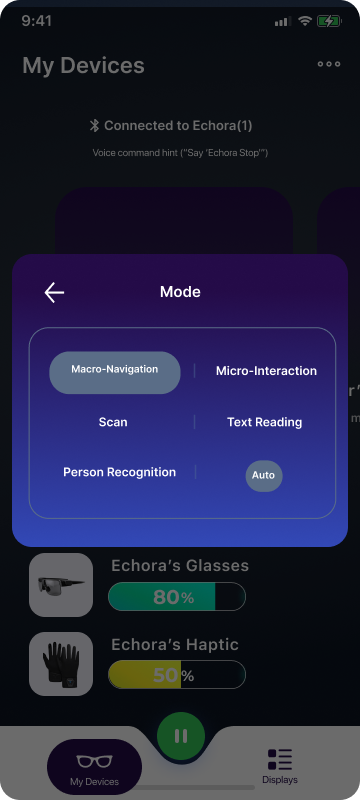
\includegraphics[width=\linewidth]{assets/Prototype/main-screen-mode.png}
\end{minipage}\hfill
\begin{minipage}[t]{0.19\textwidth}\centering
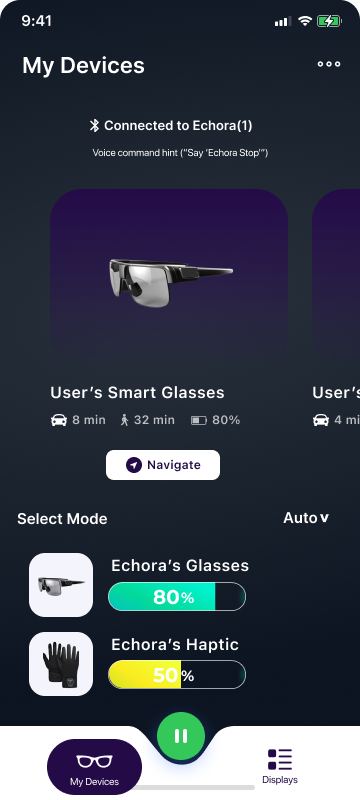
\includegraphics[width=\linewidth]{assets/Prototype/main-screen.png}
\end{minipage}\hfill
\begin{minipage}[t]{0.19\textwidth}\centering
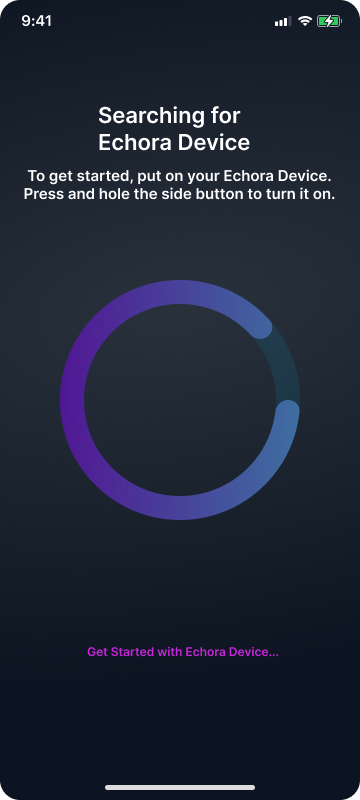
\includegraphics[width=\linewidth]{assets/Prototype/pairing-screen-2.png}
\end{minipage}

\vspace{0.6em}

% -------- Row 2 (remaining images; still same style) --------
\begin{minipage}[t]{0.19\textwidth}\centering
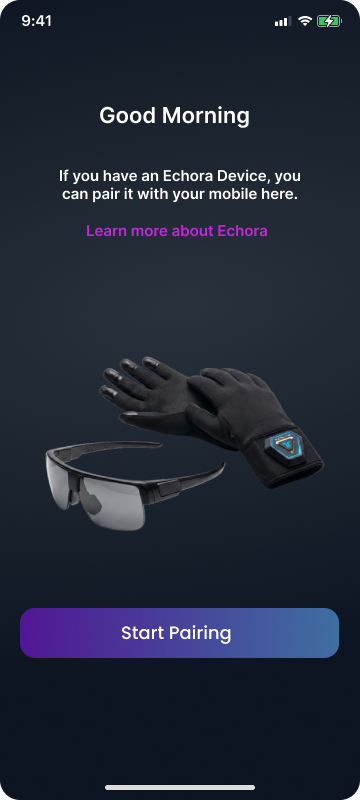
\includegraphics[width=\linewidth]{assets/Prototype/pairing-screen.png}
\end{minipage}\hfill
\begin{minipage}[t]{0.19\textwidth}\centering
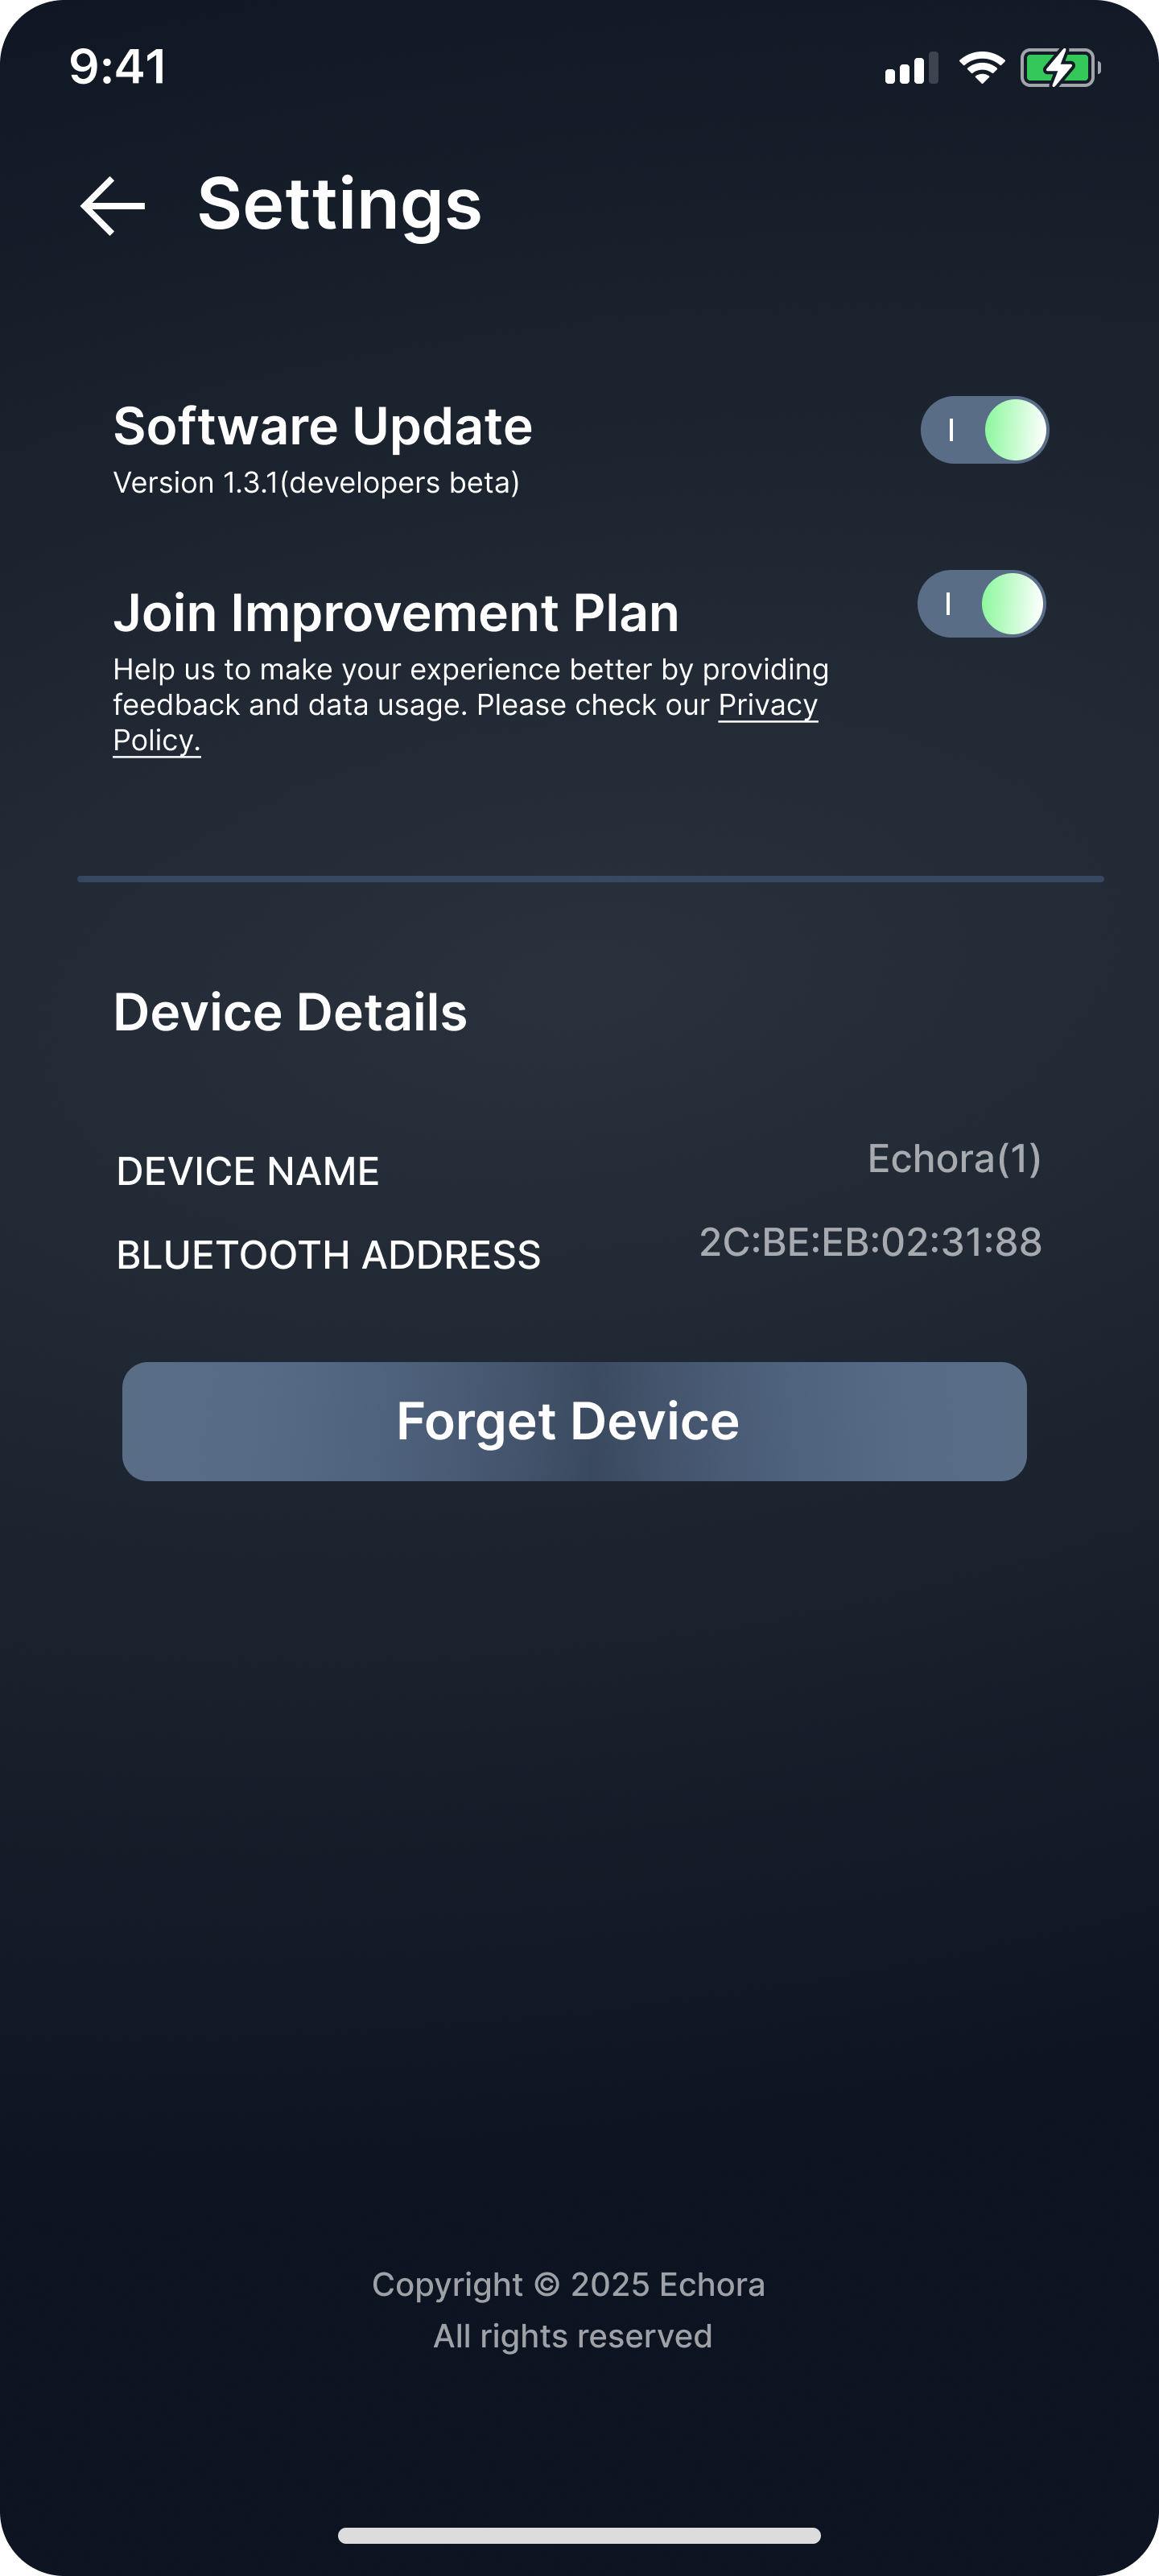
\includegraphics[width=\linewidth]{assets/Prototype/Setting Screen.png}
\end{minipage}\hfill
\begin{minipage}[t]{0.19\textwidth}\centering

\includegraphics[width=\linewidth]{assets/Prototype/Sign In.png}
\end{minipage}\hfill
\begin{minipage}[t]{0.19\textwidth}\centering

\includegraphics[width=\linewidth]{assets/Prototype/Sign Up.png}
\end{minipage}\hfill
\begin{minipage}[t]{0.19\textwidth}\centering
% empty slot to keep the row aligned to 5 columns
\end{minipage}

\caption{Echora Mobile Application Prototype Screens}
\label{fig:prototype_screens}
\end{figure}


\section{Core Algorithms and Models}

The Echora system integrates multiple lightweight artificial intelligence models optimized for real-time execution on mobile devices.

For environmental navigation, depth frames are fused with inertial measurement unit (IMU) data using a sensor fusion algorithm based on Kalman filtering. A lightweight convolutional neural network (CNN) performs real-time segmentation of walls, obstacles, humans, and open pathways. The resulting spatial information is translated into continuous spatial audio cues, where distance, direction, and urgency are encoded through volume, stereo positioning, and pitch variation.

Object interaction and hand guidance are implemented using an object detection model based on MobileNet or YOLO architectures. Detected interactive objects such as door handles and elevator panels are localized using depth measurements. Hand tracking is performed using MediaPipe Hands at a minimum of 15 frames per second. Directional correction vectors are continuously computed and translated into wrist-mounted haptic feedback until proper alignment is achieved.

Text and sign recognition is achieved through a two-stage pipeline consisting of scene text detection using EAST or DBNet models, followed by optical character recognition using a mobile-optimized Tesseract engine. Recognized text is converted into speech using an on-device TTS engine.

Critical danger detection employs time-to-collision estimation using depth difference kernels and optical flow techniques. Sudden terrain changes, such as stairs or drop-offs, are identified through ground plane discontinuity analysis. These alerts override all other system outputs to ensure immediate user safety.



\section{Implementation Challenges}

Several challenges were encountered during the implementation of the Echora system. Achieving real-time performance on mobile hardware while running multiple AI models simultaneously required careful optimization, dynamic resolution scaling, and adaptive fallback strategies.

Synchronizing heterogeneous sensor streams, including RGB, depth, and IMU data, proved challenging due to differing sampling rates and communication latencies. Timestamp-based buffering and alignment were implemented to maintain spatial consistency.

Designing effective audio and haptic feedback without overwhelming the user required extensive prioritization logic and mode management to reduce cognitive load. Additionally, mobile resource constraints such as battery consumption and thermal throttling necessitated aggressive power management and computational efficiency.

Environmental variability, including lighting changes, motion blur, and partial occlusions, also affected perception accuracy. These issues were mitigated through confidence thresholds, graceful degradation, and fallback modes.


\section{Conclusion}

This chapter presented the implementation of the Echora system using a Flutter-based mobile application as the core processing platform. The described development environment, application prototype, and AI-driven perception pipeline demonstrate the feasibility of delivering real-time, on-device sensory substitution for Blind and Low Vision users.

Despite challenges related to performance optimization, sensor reliability, and feedback design, the implemented prototype successfully integrates navigation assistance, object interaction, text recognition, and safety monitoring within a unified framework. The results validate the proposed system architecture and confirm that modern smartphones can effectively support advanced assistive technologies without reliance on cloud-based processing.

The implemented system provides a strong foundation for future enhancements, extended user testing, and potential real-world deployment.
